\documentclass[t]{beamer}
\usetheme{Warsaw}
\usecolortheme{seahorse}
\usepackage{array}
%\usepackage{graphicx}
\usepackage{amssymb,amsmath,mathrsfs,amsfonts}
%\usepackage[colorhighlight,display]{texpower}
%\usepackage{caption}
%\usepackage[all]{xy}
\usepackage{beamerthemesplit}
\mode<presentation>
%\usepackage{pause}
\usepackage{ulem}  % for strikethroughs
\usepackage{cancel} % for strikethroughs in math mode 
\usepackage{tikz}
\usetikzlibrary{shapes}
\usepackage{hyperref}
\hypersetup{pdfpagemode=FullScreen}
\usepackage{ifthen}
\usepackage{animate}
\usepackage{color}
\usepackage{type1cm}  % used for watermarking
\usepackage{eso-pic}  % used for watermarking


\theoremstyle{plain}
\newtheorem{prop}{Proposition}
\newtheorem{thm}[prop]{Theorem}
\newtheorem{lem}[prop]{Lemma}
\newtheorem{cor}[prop]{Corollary}
\theoremstyle{definition}
\newtheorem{dfn}{Definition}
\newtheorem{rem}[prop]{Remark}
\newtheorem{ex}{Example}[section]
%\newtheorem{note}{Note}[section]
\newtheorem{exercise}{Exercise}[section]
\newcommand{\nin}{\noindent}
\newcommand{\ds}{\displaystyle}
\renewcommand{\figurename}{Figure \arabic{figure}}



\renewcommand*\familydefault{\sfdefault} 




%%%%%%%%%%%%%%%%%%%%%%%%%%5
%%%%%%%%%%%%%%%%%%%%%%%%%%%%
%%%% some commands that have different meaning in the article/presentation modes

\newcommand{\vvfill}{\mode<presentation>{\vfill}  \mode<article>{\medskip}}   %vfill in presentation only
\newcommand{\sketchspace}{ 
\mode<article>{ \medskip\noindent{\textbf{Sketch:}} \vspace*{6cm} }
\mode<presentation>{ } 
}
\newcommand{\examplespace}{ 
\mode<article>{ \medskip\noindent{\textbf{Example:}} \vspace{6cm} }
\mode<presentation>{ } 
}
\newcommand{\artsmspace}{\mode<article>{\vspace*{2cm}} }  %small space in article mode
\newcommand{\artlargespace}{\mode<article>{\vspace*{6cm}} }  %large space in article mode

\newcommand{\dx}{\,dx}

\newcommand{\soln}{{\textbf{Solution: }}\,\,\,}
\newcommand{\disp}{\displaystyle}

\newcommand{\makedate}{\vvfill
\begin{picture}(10,10)  
\put(260,-20){\mbox{\tiny{\today}}}
\end{picture}
}

\newcommand{\pd}[2]{\dfrac{\partial#1}{\partial#2}}
\newcommand{\pD}[2]{\dfrac{\partial^2#1}{\partial#2^2}}
\newcommand{\pdd}[3]{\dfrac{\partial^2#1}{\partial#2 \partial#3}}


\normalem %stops the ulem package making all the emphs into underlines....
 
 
 
 \newcommand{\refandrev}[2]{
 \begin{small}
  \hspace{6cm}
  \begin{minipage}[r]{8cm}
  Stewart,    Chapter #1   \\
  Review:  \parbox[t]{6cm}{#2}
\end{minipage}
\end{small}
}



\newcounter{heading}
\setcounter{section}{1}
\setcounter{heading}{0}

\newcommand{\makeheading}[1]{\medskip\begin{large}\noindent\textbf{{#1}}\end{large}\smallskip}

%\newenvironment{head}[1]{\medskip\stepcounter{heading}\noindent\textbf{\hspace{0.2cm}{#1}.}}{}
\newcommand{\newhead}[1]{\medskip\stepcounter{heading}\noindent\textbf{\hspace{0.2cm}{#1}.}}


\newcommand{\pf}[1]{\noindent\textit{Proof.}\vspace*{#1 cm}}
\newcommand{\sol}[1]{\noindent\textit{Solution.}\vspace*{#1 cm}}
\newcommand{\further}[1]{\begin{small}\noindent\textit{Further reading: #1}\end{small}}
\newcommand{\exr}[1]{\begin{footnotesize}\noindent\textit{\textbf{Exercises:} Stewart #1}\end{footnotesize}}


% Sets of numbers
\newcommand{\C}{\mathbb{C}}
\newcommand{\RR}{\mathbb{R}}
\newcommand{\Z}{\mathbb{Z}}
\newcommand{\N}{\mathbb{N}}
\newcommand{\Q}{\mathbb{Q}}

% Partitions
\newcommand{\PP}{\mathcal{P}}

% Limits
\newcommand{\limm}[1]{\displaystyle \lim_{x\to #1}}

% Backslash
\newcommand{\bs}{\backslash}

% functions
\newcommand{\cosec}{\mathrm{cosec}}
\newcommand{\cosech}{\mathrm{cosech}}
\newcommand{\sech}{\mathrm{sech}}
\newcommand{\Li}{\mathrm{Li}}
\newcommand{\si}{\mathrm{Si}}
\newcommand{\erf}{\mathrm{erf}}

% Domain and Range
\newcommand{\Dom}{\mathrm{Dom}}
\newcommand{\Codom}{\mathrm{Codom}}
\newcommand{\Range}{\mathrm{Ran}}



\title{Week 2:  Limit and Continuity}
%\date{July 30 -- August 3, 2012}

\begin{document}

\frame{\titlepage}

\setcounter{tocdepth}{2}
\frame{\tableofcontents

%\begin{flushright}
%\hyperlink{tues}{\beamergotobutton{Lecture 4}}
%\end{flushright} 
}

\AtBeginSection[]
{
\begin{frame}<beamer> 
\tableofcontents[currentsection]  % show TOC and highlight current section
\end{frame}
}

\section{Limit}

\subsection{Limits of functions at a point}
\frame
{
  \frametitle{Meaning of  limits}
  A function may or may not be defined at a particular point, but it can have a limiting value at that point.
  
  Let us consider the function $f(x)= \ds{\frac{x^2-1}{x-1}}$.\\[3mm]
  
  \begin{tabular}{|c|c|c|c|c|}\hline
  $x$ & 0.9 & 0.999 & 1.01 & 1.0001  \\ \hline
  $\ds{\frac{x^2-1}{x-1}}$ & 1.9 & 1.999 & 2.01 & 2.0001 \\ \hline
  \end{tabular}\\[3mm]
  
  $f(x)$ is not defined at $x=1$, but as $x$ gets closer and closer to $1$, $f(x)$ gets closer and closer to $2$. 
  We say that {\em the limit of $f(x)$ as $x$ approaches to $1$, is $2$.}
  }
  
\frame
{
  \frametitle{Definition of  limits}
\begin{dfn}
The limit of $f(x)$, as $x$ approaches $a$, equals $L$ is written as
\[
\lim_{x\to a} f(x) = L \textrm{ iff } \lim_{x\to a^-} f(x) = L \textrm{ and } \lim_{x\to a^+} f(x) = L
\]
This limit \textit{exists} only if the left sided limit ($a^-$) and right sided limit ($a^+$) both exist and are equaled.   Another possible way in which limit does not exist is when $L = \pm \infty$.   Lastly, this limit does not depend whether $f(x)$ is defined or what $f(x)$ is.
\end{dfn}
}


\frame
{
	\frametitle{Rules for calculating limits}
\newhead{Basic limit rules} Suppose that $a\in\RR$ and that $\limm{a}f(x)$ and $\limm{a}g(x)$ exist and are finite real numbers. Then
\begin{enumerate}
\item[(i)] $\limm{a}(f(x)+g(x))=\limm{a}f(x)+\limm{a}g(x)$
\item[(ii)] $\limm{a}(f(x)-g(x))=\limm{a}f(x)-\limm{a}g(x)$
\item[(iii)] $\limm{a}f(x)g(x)=\limm{a}f(x)\limm{a}g(x)$
\item[(iv)] $\limm{a}\frac{f(x)}{g(x)}=\frac{\limm{a}f(x)}{\limm{a}g(x)}$,\,\, provided $\limm{a}g(x)\neq0$.
\end{enumerate}
A similar set of rules hold for left- and right-hand limits.
}

\frame
{
	\frametitle{Rules for calculating limits}

\newhead{Limit rule for compositions}\\ If $\limm{a}f(x)=L$ and $\limm{L}g(x)=g(L)$ then
\[\limm{a}g(f(x))=g\Big(\limm{a}f(x)\Big).\]

\smallskip
}


\begin{frame}

\frametitle{Rules for calculating limits}
\newhead{The squeeze theorem} Suppose that $f(x)\leq g(x)\leq h(x)$ when $x$ is near $a$ (except possibly at $a$)
and
\[\limm{a}f(x)=\limm{a}h(x)=L.\]
Then
\[\limm{a}g(x)=L.\]

\noindent (Similar versions of the squeeze theorem exist for left- and right-hand limits.)

\end{frame}
  
  

%\begin{frame}
%\newhead{The squeeze theorem for limits at infinity} Suppose that $f$, $g$ and $h$ are all defined on the interval $(b,\infty)$, where $b\in\RR$. If
%\[f(x)\leq g(x)\leq h(x)\qquad\forall x\in(b,\infty)\]
%and
%\[\limm{\infty}f(x)=\limm{\infty}h(x)=L\]
%then
%\[\limm{\infty}g(x)=L.\]
%
%\vspace*{.2cm}
%
%\newhead{Example} Use the squeeze theorem to find $\limm{\infty}\frac{\sin x}{x}$.
%
%\end{frame}

\frame
{
	\frametitle{Example}
	Describe the limit of this graph when $x$ is near 2
	
	\begin{figure}[l]
	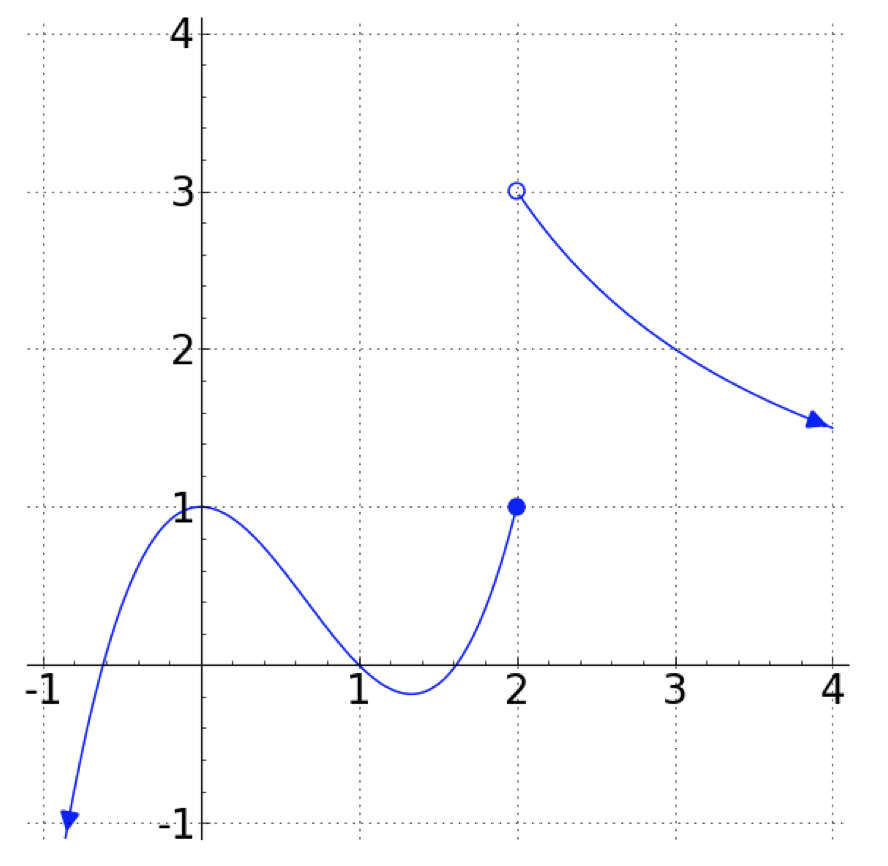
\includegraphics[scale=.3]{fig/limit0}
	\label{fig}
	\end{figure}	
	
    $\limm{2^+}f(x)=3$ \hspace{2em}
	$\limm{2^-}f(x)=1$  \hspace{2em}
	$\limm{2}f(x)=$DNE
}

\frame
{
	\frametitle{Example}
	Describe the limit of this graph when $x$ is near -2
	
	\begin{figure}[l]
	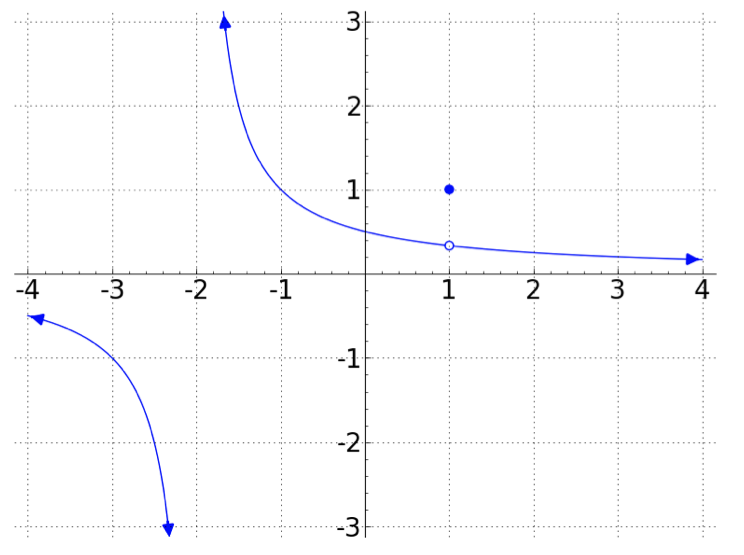
\includegraphics[scale=.2]{fig/limit1}
	\label{fig}
	\end{figure}	
	
    $\limm{-2^+}f(x)=\infty$ \hspace{2em}
	$\limm{-2^-}f(x)=-\infty$  \hspace{2em}
	$\limm{-2}f(x)=$DNE
}

\frame
{
\footnotesize

	\frametitle{Exercise}
	Describe the limit of this graph when $x$ is near -1, 1 and 2
	
	\begin{figure}[l]
	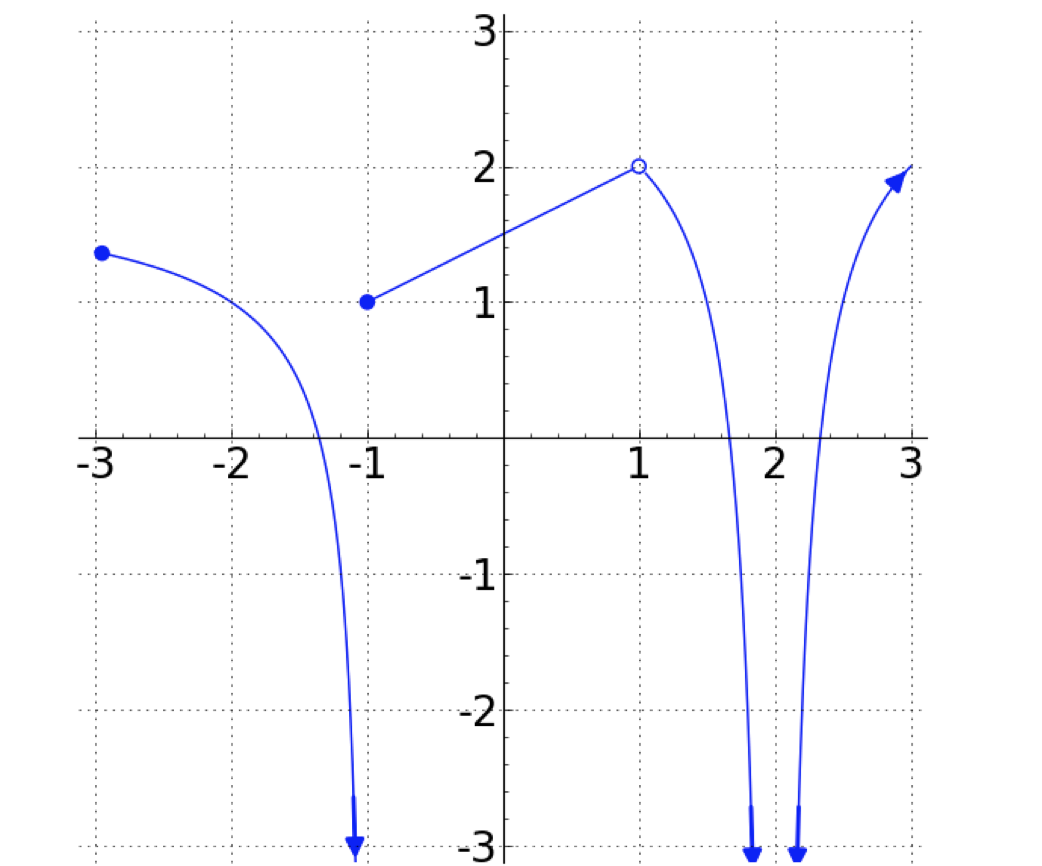
\includegraphics[scale=.28]{fig/limit2}
	\label{fig}
	\end{figure}	
	
	\pause
	
    $\limm{-1^+}f(x)=1$ \hspace{2em}
	$\limm{-1^-}f(x)=-\infty$  \hspace{2em}
	$\limm{-1}f(x)=$DNE
	
	$\limm{1^+}f(x)=2$ \hspace{3em}
	$\limm{1^-}f(x)=2$  \hspace{2.7em}
	$\limm{1}f(x)=2$
	
	$\limm{2^+}f(x)=-\infty$ \hspace{1.8em}
	$\limm{2^-}f(x)=-\infty$  \hspace{1.6em}
	$\limm{2}f(x)=-\infty$
}


\frame
{
	\frametitle{Example}
	Find $\limm{2}\dfrac{x^2 + 3x + 6}{x + 9}$
	
	\vspace{3em}

	We can directly plug in value as long as the value DOES NOT make the function undefined (based on the Limit Law).  Thus the limit is simply $\dfrac{16}{11}$
}

\frame
{
	\frametitle{Example}
	Find $\disp{\lim_{x\to 0}} \disp{\frac{|x|}{x}}$
	
	\vspace{3em}

	As $\disp{\lim_{x\to 0^+}  \frac{|x|}{x}} =1$ and $\disp{\lim_{x\to 0^-}  \frac{|x|}{x}} =-1$,
	$\disp{\lim_{x\to 0}  \frac{|x|}{x}}$ doesn't exist.

}

\frame
{
	\frametitle{Example}

Find $\disp{\lim_{x\to 1}} {\dfrac{x^2-1}{x-1}}$

\vspace{3em}

We can't find the limit by substituting $x = 1$ because $f(1)$ isn't defined.  We cannot also apply the Quotient Law,  because the limit of the denominator is 0.  Instead, we can factor the numerator:

${\dfrac{x^2-1}{x-1}=\dfrac{(x+1)(x-1)}{x-1}}= x+1$. Thus 
$\disp{\lim_{x\to 1} (x+1) = 2.}$
}



\frame
{
	\frametitle{Example}

Find $\ds\limm{0}\dfrac{1}{x^2}$

\vspace{3em}

As $x$ approaches 0 but not 0,  $f$ becomes arbitrarily large and positive, thus the limit is $\infty$ or does not exist (DNE).

}

\frame
{
	\frametitle{Example}

Find  $\ds\limm{0}f(x)=\begin{cases}
\sin(x)&\mbox{if }x\neq 0\\
5&\mbox{if }x=0
      \end{cases}$

\vspace{3em}

As $x$ approaches 0, both $\ds\limm{0^-}$ and$\ds\limm{0^+}$ are approaching 0 because $\sin(0) = 0$, thus the limit is 0 even though $f(0) = 5$.

}

\frame
{
	\frametitle{Example}

Find   $\ds\limm{4}f(x)=\begin{cases}
\sqrt{x - 4}&\mbox{if }x > 4\\
8 - 2x&\mbox{if }x=0
      \end{cases}$

\vspace{3em}

we have $\ds\limm{4^+} \sqrt{x-4} = 0$ (just substitute)

\vspace{1em}

we also have $\ds\limm{4^-} 8 - 2x = 0$  (just substitute)

\vspace{1em}

Thus the limit is 0.

}

\frame
{
	\frametitle{Example}
	Find $\limm{0}x^2\sin(\dfrac{1}{x})$ using squeeze theorem
	
	\vspace{2em}
	
    $-1 \leq \sin(\dfrac{1}{x}) \leq 1$\\
	$-x^2 \leq x^2 \sin(\dfrac{1}{x}) \leq x^2$\\
	
	\vspace{2em}
	
	Since $\limm{0}x^2 = 0$ and $\limm{0}-x^2 = 0$, thus $\limm{0}x^2\sin(\dfrac{1}{x}) = 0$

}

\frame
{
	\frametitle{Example}
	Find $\limm{3}\dfrac{2x}{x-3}$
	
	\vspace{2em}
	
    $\limm{3+}\dfrac{2x}{x-3} = \infty$ (try 3.000001)\\
    $\limm{3-}\dfrac{2x}{x-3} = -\infty$ (try 2.999999)\\
    $\limm{3}\dfrac{2x}{x-3} = $ DNE\\

}


\begin{frame}
\makeheading{Self-Exercise}
\footnotesize

\begin{enumerate}

\item $\ds{\lim_{x\to -1}} \ds{\frac{2x+2}{x+1}}$ 
\begin{itemize}
	\item Ans: $2$
\end{itemize}

\item $\limm{0} |x|$ 
\begin{itemize}
	\item Ans: $0$
\end{itemize}

\item  $\limm{-5}\dfrac{2x + 10}{|x + 5|}$
\begin{itemize}
	\item Ans: DNE because left limit is -2 and right limit is 2
\end{itemize}

\item  $\limm{1}\dfrac{\sqrt{x+3}-2}{x-1}$  \footnote{(Hint: multiply top and bottom with $\sqrt{x+3} + 2$)} 
\begin{itemize}
	\item Ans: $\dfrac{1}{4}$
\end{itemize}

\item $4\sqrt{x} \leq g(x) \leq 3x^2 - 4x + 5$.  Find limit of $g(x)$ approaching 1.
\begin{itemize}
	\item Ans: $4$
\end{itemize}

\end{enumerate}

\end{frame}

\begin{frame}
\makeheading{Self-Exercise}
\footnotesize

\begin{enumerate}

\item $\limm{6}\dfrac{x + 2}{x - 6}$
\begin{itemize}
	\item Ans: DNE because left and right limits are not the same, and also of infinities (positive and negative)
\end{itemize}

\item $\limm{-4}\dfrac{5x}{|x+4|}$
\begin{itemize}
	\item Ans: $\infty$.   Even both limits are of same sign but it is still infinity, thus DNE
\end{itemize}


\end{enumerate}

\end{frame}

\subsection{Limits at infinity}

\begin{frame}
\frametitle{Example}
	Find $\limm{\infty}\dfrac{1}{x}$
	
	\vspace{2em}
	
    As $1$ divides by a large number approaches 0, thus the limit is 0

\end{frame}

\begin{frame}
\frametitle{Example}
	Find $\limm{\infty}\dfrac{5x^2 - 4x}{2x^3 - 11x^2 + 12x}$
	
	\vspace{1em}

	We cannot just put in since we will get $\dfrac{\infty}{\infty}$.	Let's factor.
	
	\begin{align*}
  	&= \limm{\infty}\dfrac{x^2(5 - \dfrac{4}{x})}{x^3(2 - \dfrac{11}{x} + \dfrac{12}{x^2})}\\
  	&= \limm{\infty}\dfrac{1}{x} * \dfrac{5 - \dfrac{4}{x}}{2 - \dfrac{11}{x} + \dfrac{12}{x^2}} \\
  	&= \limm{\infty}0 * \dfrac{5 - 0}{2 - 0 + 0} \\
  	&= 0
	\end{align*}	
	
\end{frame}

\begin{frame}
\frametitle{Example}
	Find $\limm{-\infty}\dfrac{\sin^2{x}}{x^3}$ using squeeze theorem
	
	\begin{align*}
  	0 \leq \sin^2{x} \leq 1\\
  	0 \leq \dfrac{\sin^2{x}}{x^3} \leq \dfrac{1}{x^3}\\
	\end{align*}	
	
	Since $\limm{-\infty} 0 = 0$ and $\limm{-\infty} \dfrac{1}{x^3} = 0$, thus the limit is 0.
	
\end{frame}

\begin{frame}
\makeheading{Self-Exercise}
\footnotesize
\begin{enumerate}

\item $\limm{-\infty}\dfrac{3x^3 + 6x^2 + 10x + 2}{2x^3 + x^2 + 5}$
\begin{itemize}
	\item Ans: $\dfrac{3}{2}$
\end{itemize}

\item $\limm{-\infty}\dfrac{x^4 - 3x^2 + 6}{-5x^2 + x + 2}$
\begin{itemize}
	\item Ans: $-\infty$
\end{itemize}

\item $\limm{\infty}\dfrac{\sin{x}}{x}$  \qquad(use squeeze theorem)
\begin{itemize}
	\item Ans: $0$
\end{itemize}

\item $\limm{\infty}e^x$ 
\begin{itemize}
	\item Ans: $\infty$ or DNE
\end{itemize}

\item $\limm{\infty}\sqrt{3 + x^2} - x$  \qquad (multiply top and bottom with  $\sqrt{3 + x^2} + x$)
\begin{itemize}
	\item Ans: 0
\end{itemize}

\end{enumerate}

\end{frame}

\subsection{Special Trigonometric Limits}

\begin{frame}

\frametitle{Special Trigonometric Limits}

\begin{figure}[l]
	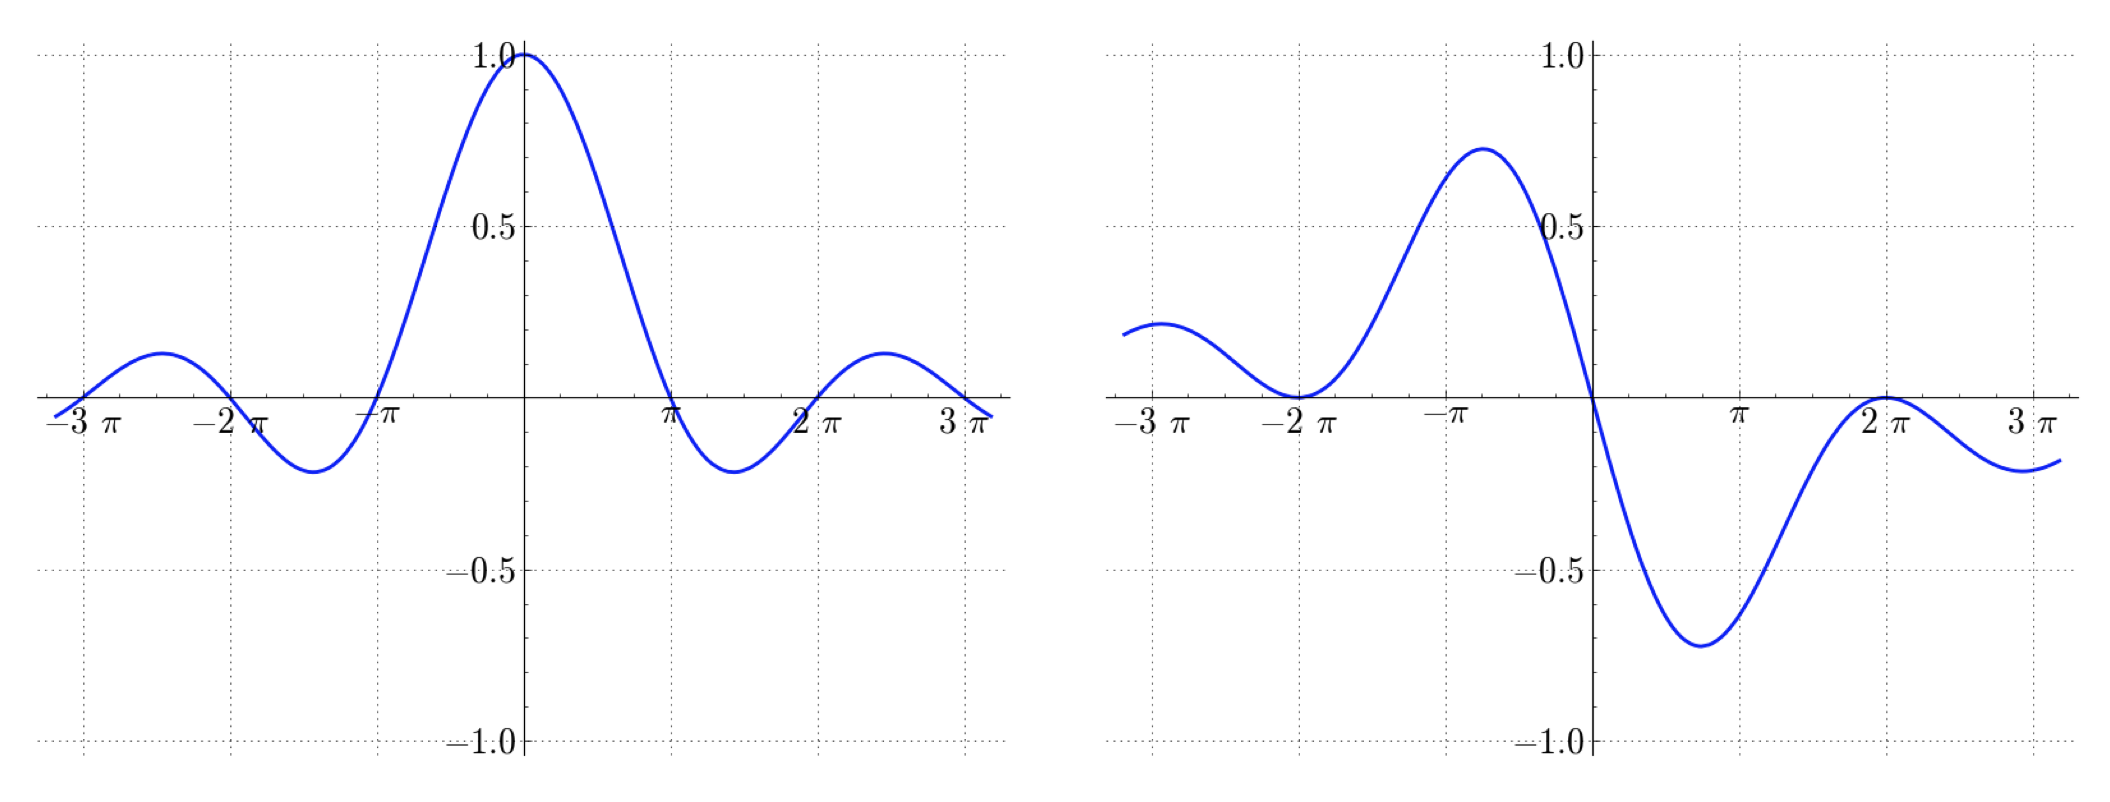
\includegraphics[scale=.25]{fig/speciallimit}
	\label{fig}
	\end{figure}	

\hspace{4em} $\disp{\lim_{\theta\to 0}  \dfrac{\sin{\theta}}{\theta}} = 1$ \hspace{7em}  $\disp{\lim_{\theta\to 0}  \dfrac{\cos{\theta}-1}{\theta}} = 0$

\vspace{2em}

Note: Given the ratio of 1, it means $\sin{\theta} \approx \theta$ when $\theta$ is near $0$

\end{frame}

\begin{frame}
\frametitle{Example}
	Find $\limm{0}\dfrac{\sin{4x}}{\sin{6x}}$
	
	\begin{align*}
  	&= \limm{0}\dfrac{\sin{4x}}{\sin{6x}}\\
  	&\approx \limm{0} \dfrac{4x}{6x}\\
  	&\approx \limm{0} \dfrac{4}{6}
	\end{align*}	

\end{frame}

\begin{frame}
\frametitle{Example}
	Find $\limm{0}\dfrac{\tan{7x}}{\sin{4x}}$
	
	\begin{align*}
  	&= \limm{0}\dfrac{\dfrac{\sin{7x}}{\cos{7x}}}{\sin{4x}}\\
  	&= \limm{0}\dfrac{\sin{7x}}{\cos{7x}} * \dfrac{1}{\sin{4x}}\\
  	&\approx \limm{0}\dfrac{7x}{\cos{7x}} * \dfrac{1}{4x}\\
  	&\approx \dfrac{7}{4}\limm{0}\dfrac{1}{\cos{7x}}\\
  	&\approx \dfrac{7}{4}
	\end{align*}	

\end{frame}


%
%\begin{frame}
%\uncover<+->{\noindent We have a similar definition for the limit as $x$ goes to $-\infty$:
%
%\noindent Let $f$ be a function defined on some interval $(-\infty, a)$ or $(-\infty, \infty)$.  Then 
%\[\lim_{x\rightarrow -\infty}f(x) = L\]
%means that the values of $f(x)$ can be made arbitrarily close to $L$ by taking $x$ sufficiently large and negative.}
%
%\uncover<+->{\vspace*{.1cm}
%\newhead{Question} What is the value of $\limm{-\infty} e^{x}$?}
%
%\uncover<+->{\vspace*{.1cm}
%
%\noindent The line $y=L$ is called a \emph{horizontal asymptote} of the curve $y = f(x)$ if either 
%\[ \lim_{x\rightarrow \infty}f(x) = L \qquad \text{or} \qquad \lim_{x\rightarrow -\infty}f(x) = L.\]}
%\end{frame}
%
%\begin{frame}
%\newhead{Basic rules} Suppose that $\limm{\infty}f(x)$ and $\limm{\infty}g(x)$ exist and are \underline{finite} real numbers. Then
%\begin{enumerate}[<+->]
%\item[(i)] $\limm{\infty}[f(x)+g(x)]=\limm{\infty}f(x)+\limm{\infty}g(x)$
%\item[(ii)] $\limm{\infty}[f(x)-g(x)]=\limm{\infty}f(x)-\limm{\infty}g(x)$
%\item[(iii)] $\limm{\infty}[f(x)g(x)]=[\limm{\infty}f(x)][\limm{\infty}g(x)]$
%\item[(iv)] $\limm{\infty}\frac{f(x)}{g(x)}=\frac{\limm{\infty}f(x)}{\limm{\infty}g(x)}$, provided $\limm{\infty}g(x)\neq0$.
%\item[(v)] if $\limm{\infty}f(x) = \infty$, then $\limm{\infty}\frac{1}{f(x)}= 0$.
%\end{enumerate}
%
%\vspace*{.2cm}
%
%\uncover<+->{\newhead{Examples}}
%\begin{enumerate}[<+->]
%\item[(a)]$\limm{\infty}(\frac{1}{x} + 1 - e^{-2x})$
%\item[(b)]$\limm{-\infty}(\frac{3}{x} + 1 - cos(x))$ 
%\end{enumerate}
%\end{frame}

%
%\begin{frame}
%\newhead{Indeterminate forms}
%
%\noindent Limits of the type
%\[\limm{\infty}\frac{f(x)}{g(x)}\]
%where $f(x)\to\infty$ and $g(x)\to\infty$ as $x\to\infty$ are said to be limits of the form $\frac{\infty}{\infty}$.
%While the following limits have the form $\frac{\infty}{\infty}$, each displays very different limiting behavior as $x\to\infty$:
%\begin{itemize}
%\item $\qquad$ $\limm{\infty}\frac{x}{x}$
%\item $\qquad$ $\limm{\infty}\frac{x}{x^{2}}$
%\item $\qquad$ $\limm{\infty}\frac{x^{3}}{x}$
%\item $\qquad$ $\limm{\infty}\frac{e^{x}}{x}$ $\qquad$ (deal with this more later)
%\end{itemize}
%
%\end{frame}


%\section*{Limits at infinity}
%\begin{frame}
%\newhead{Indeterminate forms}
%
%\uncover<+->{\noindent Limits of the type
%\[\limm{\infty}\frac{f(x)}{g(x)}\]
%where $f(x)\to\infty$ and $g(x)\to\infty$ as $x\to\infty$ are said to be limits of the form $\frac{\infty}{\infty}$.}
%\uncover<+->{While the following limits have the form $\frac{\infty}{\infty}$, each displays very different limiting behavior as $x\to\infty$:}
%\begin{itemize}[<+->]
%\item $\qquad$ $\limm{\infty}\frac{x}{x}$
%\item $\qquad$ $\limm{\infty}\frac{x}{x^{2}}$
%\item $\qquad$ $\limm{\infty}\frac{x^{3}}{x}$
%\item $\qquad$ $\limm{\infty}\frac{e^{x}}{x}$ $\qquad$ (deal with this more later)
%\end{itemize}
%
%\end{frame}
%
%\begin{frame}
%\uncover<+->{Since we cannot determine in advance what kind of limiting behavior something of the form $\frac{\infty}{\infty}$ has, we say that $\frac{\infty}{\infty}$ is an \textit{indeterminate form}.  Note that $\infty-\infty$ and $\frac{0}{0}$ are also indeterminate forms. }
%
%\uncover<+->{\newhead{Limits of the form $f(x)/g(x)$}
%To calculate a limit of the form
%\[\limm{\infty}\frac{f(x)}{g(x)}\]
%where both $f(x)$ and $g(x)$ tend to infinity as $x\to\infty$, one approach is to divide both $f$ and $g$ by the \textit{fastest growing term} appearing in the denominator $g$.}
%
%\uncover<+->{\newhead{Examples} }
%\begin{enumerate}[<+->]
%\item Evaluate $\limm{\infty}\frac{3x^2-x+1}{7+6x^2}$.
%\item Find $\limm{\infty}\frac{x^2+3x}{\sqrt{2x^4+3}-4x}$.
%\end{enumerate} 
%\end{frame}
%
%\begin{frame}
%\newhead{Limits of the form $\sqrt{f(x)}-\sqrt{g(x)}$} The trick is to multiply both numerator and denominator by the `conjugate squared,' and then expand the numerator as a difference of squares.\pause
%
%
%\vspace*{.4cm}
%
%\newhead{Example}
%Evaluate $\limm{\infty}\big(\sqrt{x^2+x}-x\big)$, if it exists.
%
%\end{frame}

\section{Continuity}
\subsection{Continuous functions}
\begin{frame}
\frametitle{Continuous functions}
\begin{dfn} Suppose that $f$ is defined on some open interval containing the point $a$. If
\[\limm{a}f(x) = f(a) \]
then we say that $f$ is \textit{continuous} at $a$; otherwise, we say that $f$ is \textit{discontinuous} at $a$.  Continuity can also be described from only one side as follows:
\[\limm{a-}f(x) = f(a) \]
\[\limm{a+}f(x) = f(a) \]
\end{dfn}


\end{frame}

\begin{frame}
\frametitle{Example}

What are places where $f$ is not continuous and why?

	\begin{figure}[l]
	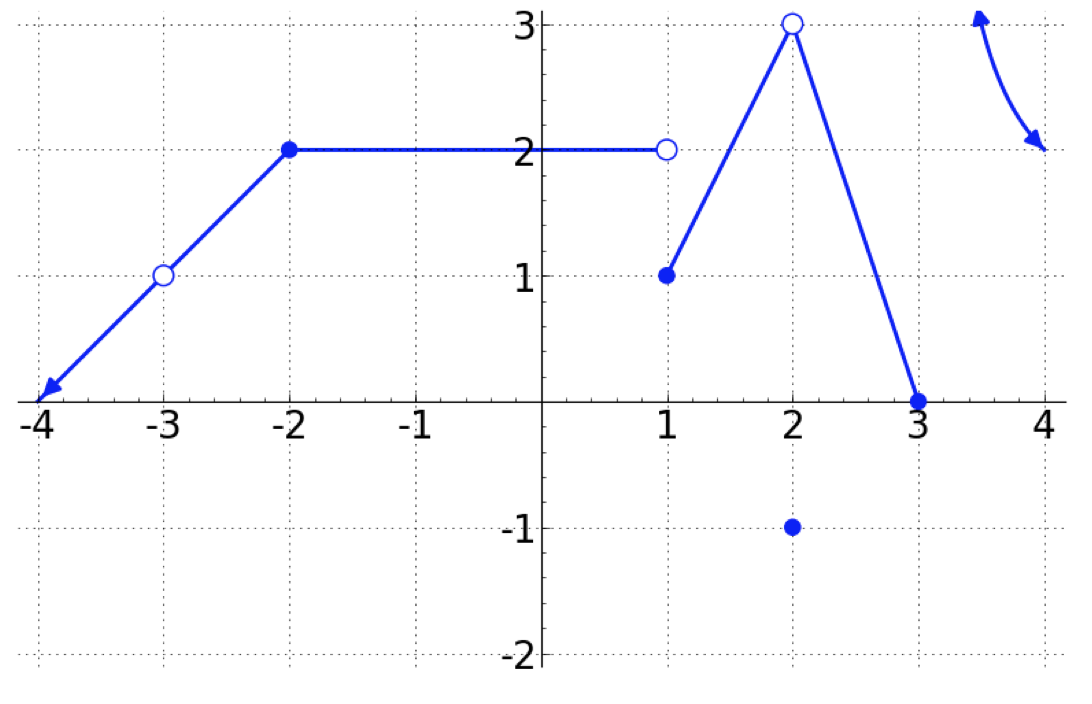
\includegraphics[scale=.3]{fig/con0}
	\label{fig}
	\end{figure}	
	
-3 because $f(-3)$ DNE\\
1 because $\limm{1}f(x)$ DNE\\
2 because $\limm{2}f(x) \neq f(2)$\\
3 because $\limm{3}f(x)$ DNE\\

\end{frame}

\begin{frame}
\frametitle{Example}

Is it continuous at $x=-2$ and $x=1$?  How about one-sided continuity?
	\begin{figure}[l]
	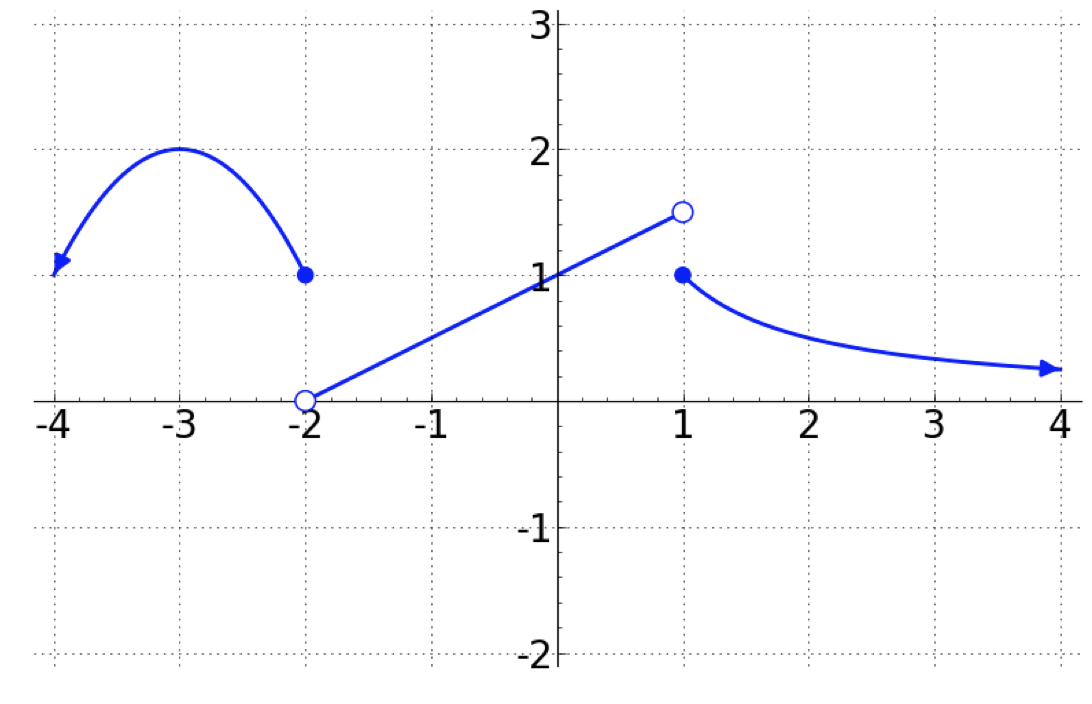
\includegraphics[scale=.25]{fig/con1}
	\label{fig}
	\end{figure}	
	
not cont. at $x = -2$ because $\limm{-2^+} \neq \limm{-2^-}$ thus limit DNE\\
cont at $x = -2^-$ because $\limm{-2^-} = f(-2) = 1$\\

not cont. at $x = 1$ because$\limm{2^+} \neq \limm{1^-}$ thus limit DNE\\
 cont at $x = 1^+$ because $\limm{2^+} = f(1) = 1$\\

\end{frame}

\begin{frame}
\frametitle{Exercise}
Which point is NOT continuous?  (both side)
	\begin{figure}[l]
	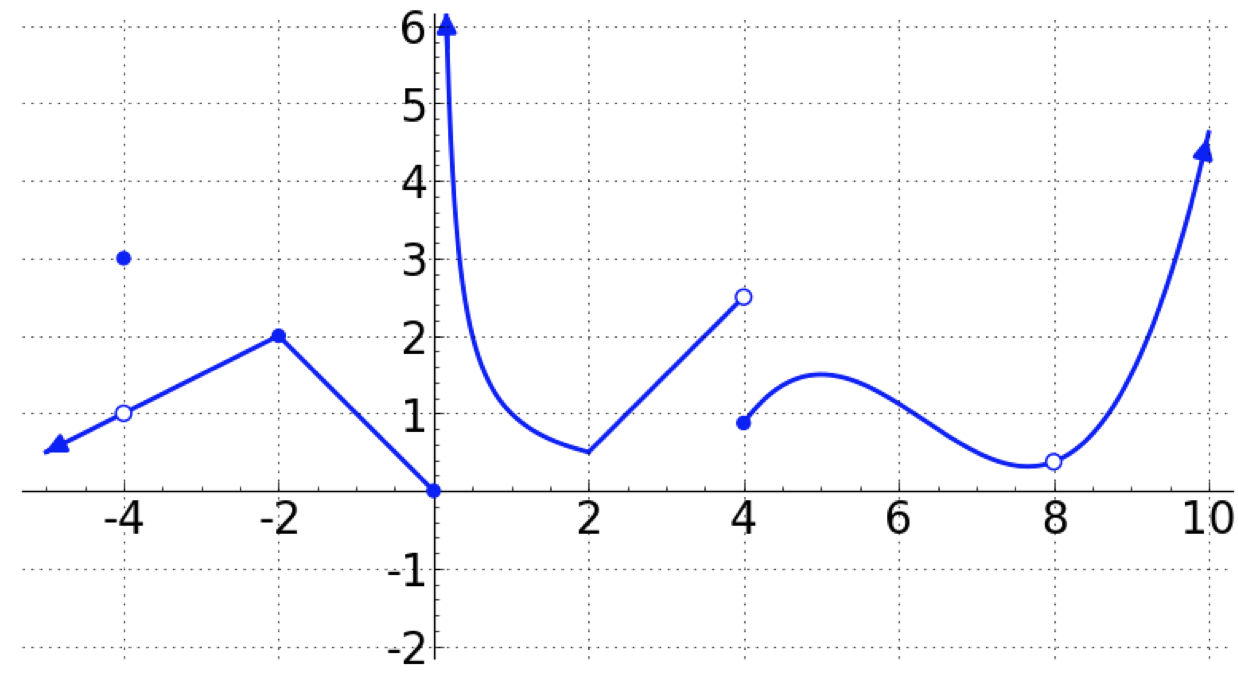
\includegraphics[scale=.4]{fig/con2}
	\label{fig}
	\end{figure}	
	\pause
Ans: -4 (limit $\neq f$), 0 (limit DNE), 4 (limit DNE), 8 (f(8) DNE)
\end{frame}

\begin{frame}
\frametitle{Exercise}
Which point is continuous from the (1) right and (2) left? 
	\begin{figure}[l]
	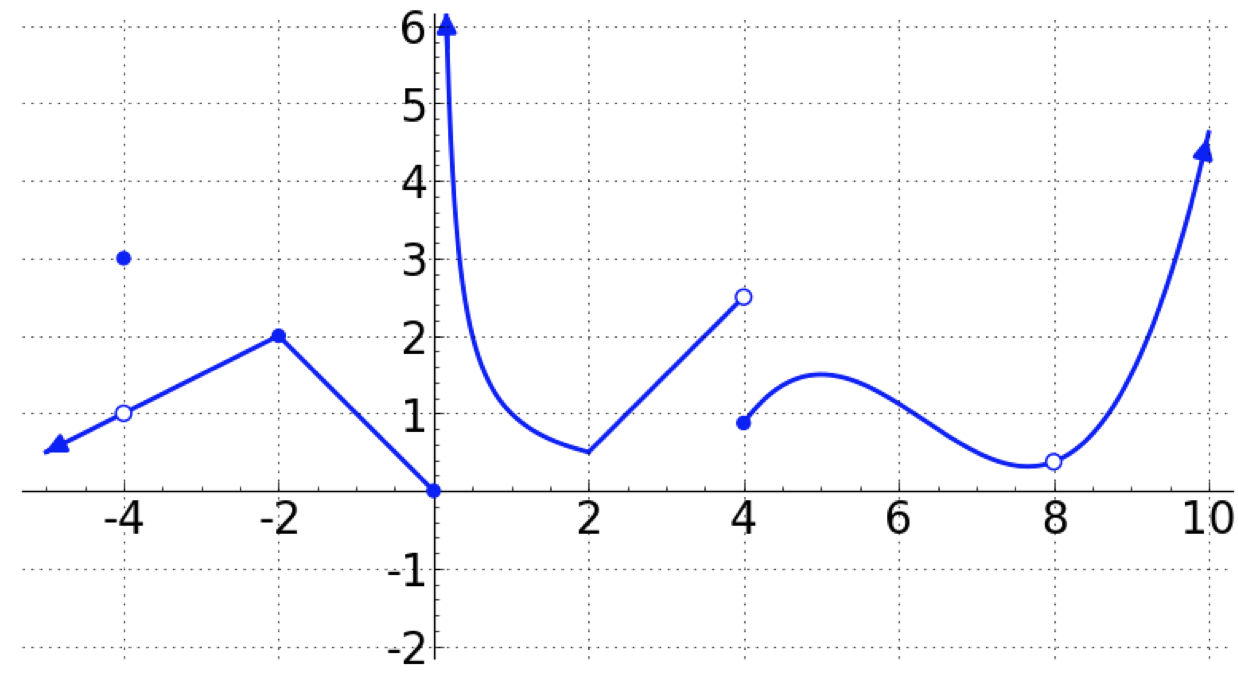
\includegraphics[scale=.4]{fig/con2}
	\label{fig}
	\end{figure}	
	\pause
Right: $4^+$ ; Left: $0^-$
\end{frame}

\begin{frame}
\frametitle{Continuous functions at intervals}

\begin{dfn}
Suppose that $f$ is a real-valued function defined on an \textbf{open} interval $(a,b)$. We say that $f$ is a \textit{continuous on $(a,b)$} if $f$ is continuous at every point in the interval $(a,b)$.
\end{dfn}

\begin{dfn}
Suppose that $f$ is a real-valued function\\ defined on a \textbf{closed} interval $[a,b]$. We say that
\begin{enumerate}
\item[(a)] $f$ is continuous at the endpoint $a$ if $\limm{a^+}f(x)=f(a)$,
\item[(b)] $f$ is continuous at the endpoint $b$ if $\limm{b^-}f(x)=f(b)$,
\item[(c)] $f$ is continuous on the closed interval $[a,b]$ if $f$ is continuous on the open interval $(a,b)$ and at each of the endpoints $a$ and $b$.
\end{enumerate}
\end{dfn}

\end{frame}

\begin{frame}
\frametitle{Combining continuous functions}

\begin{prop} Suppose that the functions $f$ and $g$ are continuous at a point $a$. Then $f+g$, $f-g$ and $fg$ are continuous at $a$. If $g(a)\neq0$ then $f/g$ is also continuous at $a$.\end{prop}

\begin{prop} Suppose that $f$ is continuous at $a$ and that $g$ is continuous at $f(a)$. Then $g\circ f$ is continuous at $a$.\end{prop}

\begin{cor} Suppose that $f$ and $g$ are continuous on their domains and that $\limm{a}f(x)$ belongs to $\Dom(g)$. Then\vspace*{-.4 cm}
\[\vspace*{-.4 cm}\limm{a}g(f(x))=g\big(\limm{a}f(x)\big).\]
(\emph{``you can move limits inside continuous functions''})\end{cor}
\end{frame}

%\begin{frame}
%\frametitle{Combining continuous functions}
%
%\newhead{Example} Suppose that $a$ and $b$ are real numbers and consider the function $f$ with domain $\RR$ given by
%\[
%f(x)=
%\begin{cases}
%x^2-a^2&\mbox{if }x<0\\
%\cos x+b &\mbox{if }x\geq0.
%\end{cases}
%\]
%For what values of $a$ and $b$ will $f$ be continuous at $0$?
%\end{frame}

\subsection{The intermediate value theorem}
\begin{frame}[label=tues]
\frametitle{The intermediate value theorem (IVT)}

\uncover<+->{
\begin{theorem}[The intermediate value theorem] 
Suppose that $f$ is continuous on the closed interval $[a,b]$. If $z$ lies between $f(a)$ and $f(b)$ then there is at least one real number $c$ in $[a,b]$ such that $f(c)=z$.
\end{theorem}}

\uncover<+->{\newhead{Example} Show that if $f(x)$ is continuous on $[0, 4]$ and $f(0)=5$ and $f(4)=1$, then $f(a) = \sqrt{2}$ for some number $a$

\vspace{2em}

Since $5 < \sqrt{2} < 1$, thus $f(a) = \sqrt{2}$ for some number $a$, according to the IVT theorem.

}


\end{frame}


\end{document}